\documentclass[Arkitektur/System_main.tex]{subfiles}
\begin{document}
\subsection{Development View}
\subsubsection{Introduktion}
I dette afsnit beskrives development view for applikationen. Formållet med dette view er at få overblik over hele applikationen, hvor de forskellige applikations lag er vist med tilhørende moduler samt forbindelser mellem dem. Til dette er der lavet et model diagram for en multi-layered applikation, som kan ses på figur \ref{fig:PackageDiagram}. I diagrammet ses en stiplet linje de steder, hvor en forbindelse går gennem wpf frameworket. De faste linjer beskriver forbindelser, der gruppen har lavet. Et eksempel på et sted, hvor en stiplet linje er brugt er til og og fra modulet databinding. Databinding er noget, der foregår igennem wpf frameworket og er ikke noget gruppen har lavet.

\begin{figure}[H]
    \centering
    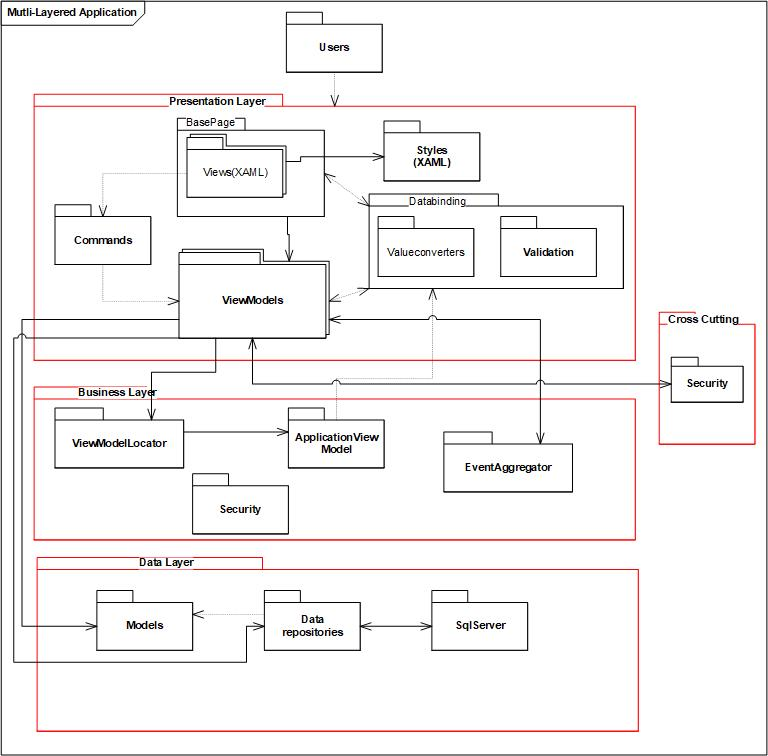
\includegraphics[width=\textwidth]{Arkitektur/4+1View/Graphics/PackageDiagram.jpg}
    \caption{Model diagram for Multi-Layered Applikation}
    \label{fig:PackageDiagram}
\end{figure}

\end{document}